
\documentclass[a4paper,11pt]{article}
\usepackage[a4paper, margin=8em]{geometry}

% usa i pacchetti per la scrittura in italiano
\usepackage[french,italian]{babel}
\usepackage[T1]{fontenc}
\usepackage[utf8]{inputenc}
\frenchspacing 

% usa i pacchetti per la formattazione matematica
\usepackage{amsmath, amssymb, amsthm, amsfonts}

% usa altri pacchetti
\usepackage{gensymb}
\usepackage{hyperref}
\usepackage{standalone}

% imposta il titolo
\title{Appunti Comunicazioni Numeriche}
\author{Luca Seggiani}
\date{2026}

% imposta lo stile
% usa helvetica
\usepackage[scaled]{helvet}
% usa palatino
\usepackage{palatino}
% usa un font monospazio guardabile
\usepackage{lmodern}

\renewcommand{\rmdefault}{ppl}
\renewcommand{\sfdefault}{phv}
\renewcommand{\ttdefault}{lmtt}

% disponi il titolo
\makeatletter
\renewcommand{\maketitle} {
	\begin{center} 
		\begin{minipage}[t]{.8\textwidth}
			\textsf{\huge\bfseries \@title} 
		\end{minipage}%
		\begin{minipage}[t]{.2\textwidth}
			\raggedleft \vspace{-1.65em}
			\textsf{\small \@author} \vfill
			\textsf{\small \@date}
		\end{minipage}
		\par
	\end{center}

	\thispagestyle{empty}
	\pagestyle{fancy}
}
\makeatother

% disponi teoremi
\usepackage{tcolorbox}
\newtcolorbox[auto counter, number within=section]{theorem}[2][]{%
	colback=blue!10, 
	colframe=blue!40!black, 
	sharp corners=northwest,
	fonttitle=\sffamily\bfseries, 
	title=~\thetcbcounter: #2, 
	#1
}

% disponi definizioni
\newtcolorbox[auto counter, number within=section]{definition}[2][]{%
	colback=red!10,
	colframe=red!40!black,
	sharp corners=northwest,
	fonttitle=\sffamily\bfseries,
	title=~\thetcbcounter: #2,
	#1
}

% U.D.M
\newcommand{\amp}{\ensuremath{\mathrm{A}}}
\newcommand{\volt}{\ensuremath{\mathrm{V}}}
\newcommand{\meter}{\ensuremath{\mathrm{m}}}
\newcommand{\second}{\ensuremath{\mathrm{s}}}
\newcommand{\farad}{\ensuremath{\mathrm{F}}}
\newcommand{\henry}{\ensuremath{\mathrm{H}}}
\newcommand{\siemens}{\ensuremath{\mathrm{S}}}

% circuiti
\usepackage{circuitikz}
\usetikzlibrary{babel}

% disegni
\usepackage{pgfplots}
\pgfplotsset{width=10cm,compat=1.9}

% disponi codice
\usepackage{listings}
\usepackage[table]{xcolor}

\lstdefinestyle{codestyle}{
		backgroundcolor=\color{black!5}, 
		commentstyle=\color{codegreen},
		keywordstyle=\bfseries\color{magenta},
		numberstyle=\sffamily\tiny\color{black!60},
		stringstyle=\color{green!50!black},
		basicstyle=\ttfamily\footnotesize,
		breakatwhitespace=false,         
		breaklines=true,                 
		captionpos=b,                    
		keepspaces=true,                 
		numbers=left,                    
		numbersep=5pt,                  
		showspaces=false,                
		showstringspaces=false,
		showtabs=false,                  
		tabsize=2
}

\lstdefinestyle{shellstyle}{
		backgroundcolor=\color{black!5}, 
		basicstyle=\ttfamily\footnotesize\color{black}, 
		commentstyle=\color{black}, 
		keywordstyle=\color{black},
		numberstyle=\color{black!5},
		stringstyle=\color{black}, 
		showspaces=false,
		showstringspaces=false, 
		showtabs=false, 
		tabsize=2, 
		numbers=none, 
		breaklines=true
}

\lstdefinelanguage{javascript}{
	keywords={typeof, new, true, false, catch, function, return, null, catch, switch, var, if, in, while, do, else, case, break},
	keywordstyle=\color{blue}\bfseries,
	ndkeywords={class, export, boolean, throw, implements, import, this},
	ndkeywordstyle=\color{darkgray}\bfseries,
	identifierstyle=\color{black},
	sensitive=false,
	comment=[l]{//},
	morecomment=[s]{/*}{*/},
	commentstyle=\color{purple}\ttfamily,
	stringstyle=\color{red}\ttfamily,
	morestring=[b]',
	morestring=[b]"
}

% disponi sezioni
\usepackage{titlesec}

\titleformat{\section}
	{\sffamily\Large\bfseries} 
	{\thesection}{1em}{} 
\titleformat{\subsection}
	{\sffamily\large\bfseries}   
	{\thesubsection}{1em}{} 
\titleformat{\subsubsection}
	{\sffamily\normalsize\bfseries} 
	{\thesubsubsection}{1em}{}

% disponi alberi
\usepackage{forest}

\forestset{
	rectstyle/.style={
		for tree={rectangle,draw,font=\large\sffamily}
	},
	roundstyle/.style={
		for tree={circle,draw,font=\large}
	}
}

% disponi algoritmi
\usepackage{algorithm}
\usepackage{algorithmic}
\makeatletter
\renewcommand{\ALG@name}{Algoritmo}
\makeatother

% disponi numeri di pagina
\usepackage{fancyhdr}
\fancyhf{} 
\fancyfoot[L]{\sffamily{\thepage}}

\makeatletter
\fancyhead[L]{\raisebox{1ex}[0pt][0pt]{\sffamily{\@title \ \@date}}} 
\fancyhead[R]{\raisebox{1ex}[0pt][0pt]{\sffamily{\@author}}}
\makeatother

\begin{document}
% sezione (data)
\section{Lezione del 19-03-26}

% stili pagina
\thispagestyle{empty}
\pagestyle{fancy}

% testo
In 5.2.1 abbiamo visto la \textit{composizione} degli esperimenti, e considerato la funzione \textit{probabilità} nel caso di esperimenti assunti \textit{indipendenti}. Vediamo cosa succede se l'ipotesi di indipendenza viene meno.

\subsection{Composizione di esperimenti non indipendenti}
Posto un esperimento composto da esperimenti sugli spazi campione $\Omega_1$, $\Omega_2$, questi si dicono \textbf{dipendenti} se l'esecuzione del primo esperimento (sullo spazio $\Omega_1$ modifica lo spazio $\Omega_2$.

In questo caso il metodo di risoluzione varia di problema in problema. Di sicuro, una soluzione che possiamo adottare è quello di considerare il primo esperimento, e valutare il risultato del secondo esperimento in funzione del risultato del primo.

\subsubsection{Canale di comunicazione binario simmetrico}
Facciamo un esempio pratico. Prendiamo un canale di comunicazione che può trasmettere segnali binari ($0$ o $1$). Poniamo che:
\begin{itemize}
	\item $1$ viene trasmesso con probabilità $p = 0.3$ e 0 con probabilità $1 - p = 0.7$;
	\item Si ha una probabilità di errore $P_e = 0.01$ sul singolo bit (indipendentemente dal simbolo trasmesso).
\end{itemize}

Ciò che vogliamo valutare è, ricevuto il bit 0, la probabilità che questo sia stato effettivamente trasmesso.
Definiamo una serie di eventi:
\begin{itemize}
	\item $T_0$ come l'evento di \textit{trasmissione} di $0$;
	\item $T_1$ come l'evento di \textit{trasmissione} di $1$;
	\item $R_0$ come l'evento di \textit{ricezione} di $0$;
	\item $R_1$ come l'evento di \textit{ricezione} di $1$;
\end{itemize}
In funzione di tali eventi, ciò che vogliamo valutare è la probabilità \textit{condizionata} (vista in 5.1):
$$
P[T_0 | R_0]
$$

Possiamo visualizzare le proprietà su un grafico, ponendo gli stati $S_0$ e $S_1$ (rispettivamente, inviato $0$ o $1$):
\begin{center}
	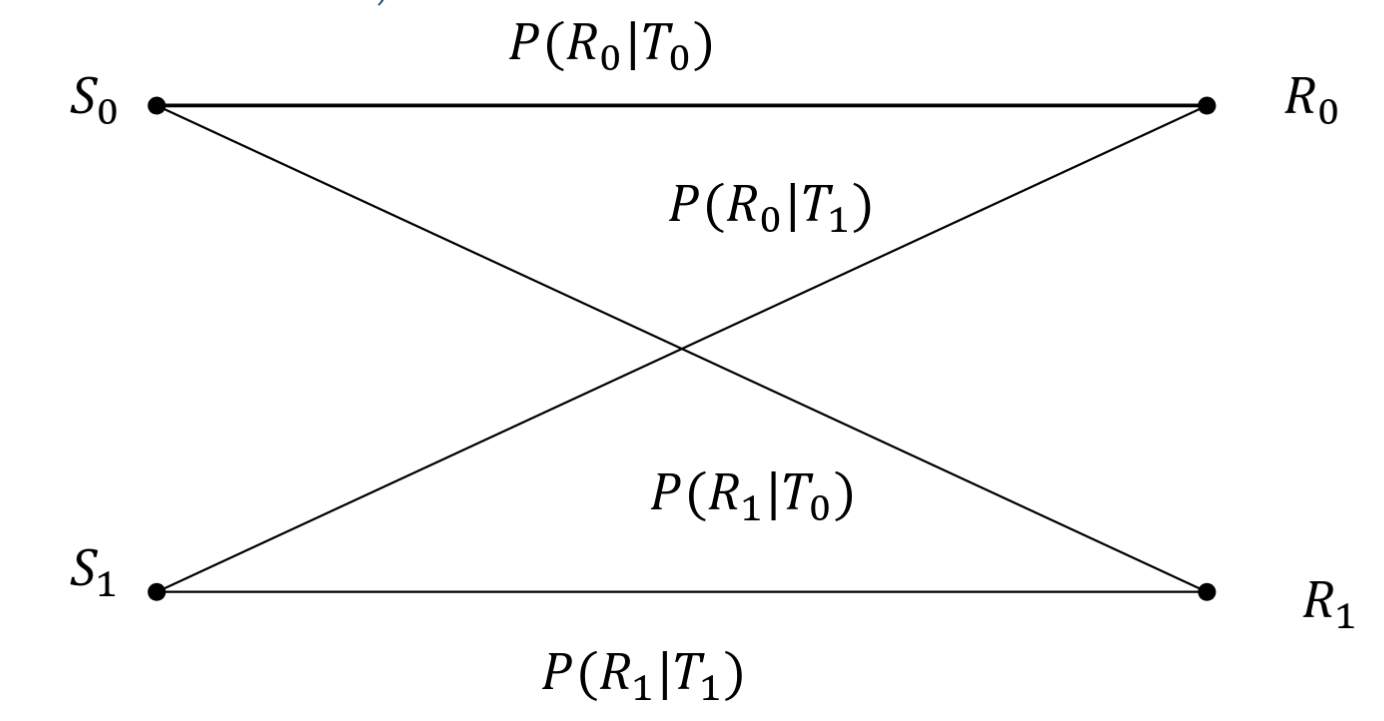
\includegraphics[scale=0.3]{../figures/channel_trans.png}
\end{center}

Il sistema è quindi concettualizzabile come due esperimenti separati ma dipendenti, dove in particolare:
$$
\begin{cases}
	\Omega_1 = \{ S_0, S_1 \} \\
	\Omega_2 = \{ R_0, R_1 \} \\
\end{cases}
\implies
\Omega = \{
	(T_0, R_0),
	(T_0, R_1),
	(T_1, R_0),
	(T_1, R_1),
\}
$$

Possiamo quindi applicare il teorema di \textit{Bayes} (5.5) per trovare quanto richiesto, ponendo:
$$
P[T_0 | R_0] = \frac{P[R_0 | T_0] P (T_0)}{P(R_0)}
$$

\begin{itemize}
\item Per il valore $P[R_0 | T_0 ]$ abbiamo che la probabilità di errore sarà data da:
$$
P_e = P[R_0 | T_1] = P[R_1 | T_0] = 0.01
$$
da cui si può ricavare la probabilitò di ricezione corretta:
$$
P[R_0 | T_0] = 1 - P[R_1 | T_0] = 0.99
$$

\item Quindi conosciamo $P(T_0)$ che è uguale a $0.7$;
	
\item Infine, per trovare $P(R_0)$ si applicherà il teorema della probabilità totale (5.4):
$$
P(R_0) = P[R_0 | T_0] P(T_0) + P[R_0 | T_1] P(T_1) = 0.99 \cdot 0.7 + 0.01 \cdot 0.3 = 0.696
$$
\end{itemize}

Prendiamo quindi il risultato finale:
$$
P[T_0 | R_0] = \frac{0.99 \cdot 0.7}{0.696} \approx 0.996
$$

\par\smallskip

\noindent
\textbf{\textsf{Caso generale}}

\noindent
Generalizzando $P_e$ ad un valore qualsiasi (quindi ricezione corretta su $p = 1 - P_e$) e la probabilità che si trasmetta $1$ ad $\alpha$ (quindi $0$ su $p' = 1 - \alpha$), otteniamo:
\begin{itemize}
\item Per il valore $P[R_0 | T_0 ]$  abbiamo che la probabilità di errore sarà data da:
$$
P_e = P[R_0 | T_1] = P[R_1 | T_0] = P_e 
$$
da cui si può ricavare la probabilitò di ricezione corretta:
$$
P[R_0 | T_0] = 1 - P[R_1 | T_0] = (1 - P_e) 
$$

\item Quindi conosciamo $P(T_0)$ che è uguale a $1 - \alpha$;
	
\item Infine, per trovare $P(R_0)$ si applicherà il teorema della probabilità totale:
$$
P(R_0) = P[R_0 | T_0] P(T_0) + P[R_0 | T_1] P(T_1) = (1 - P_e) \cdot (1- \alpha) + P_e \cdot \alpha 
$$
\end{itemize}

Prendiamo quindi il risultato finale:
$$
P[T_0 | R_0] = \frac{(1 - P_e) (1 - \alpha)}{(1 - P_e) \cdot (1 - \alpha) + P_e \cdot \alpha} = \frac{1}{1 + \frac{P_e \cdot \alpha}{(1 - P_e) (1 - \alpha)}}
$$

\newpage

Mantenuto $\alpha = 0.3$, tracciamo un grafico di $P[T_O | R_0]$ in funzione di $P_e$:
\begin{center}
	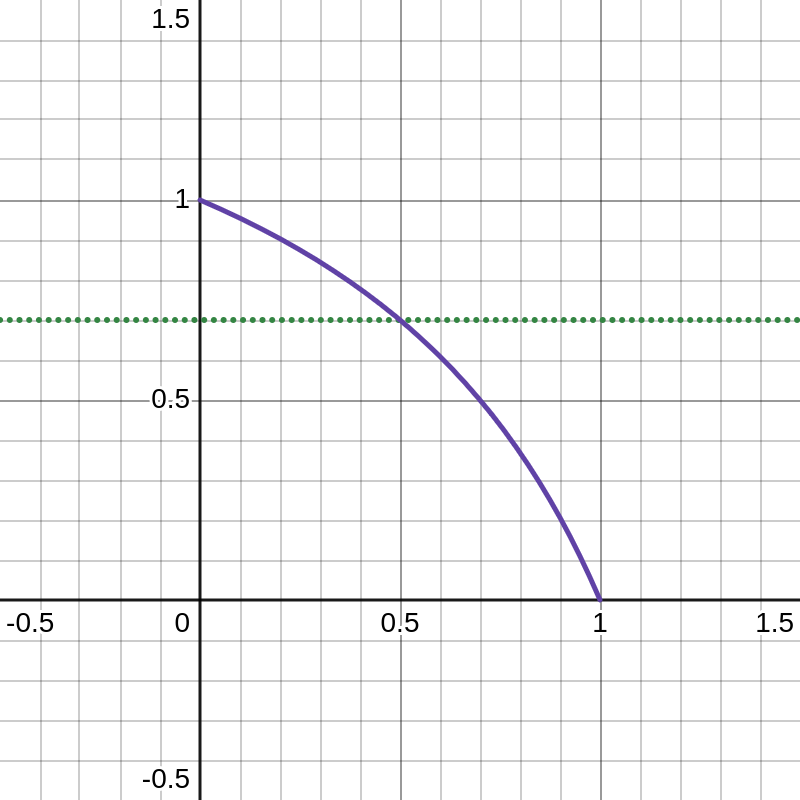
\includegraphics[scale=0.25]{../figures/bin_chan_prob.png}
\end{center}

Da questo grafico, notiamo alcuni valori particolari:
\begin{itemize}
	\item Per $P_e = 0$, la probabilità è piena, cioè possiamo fidarci pienamente del mezzo (non c'è possibilità di errore);
	\item Per $P_e = \frac{1}{2}$, cioè errori completamente aleatori, il meglio che possiamo assicurare è la probabilità:
$$P[T_0 | R_0] = 1 - \alpha = P(T_0)$$
cioè la possibilità che $T_0$ si sia effettivamente verificato dato il segnale $R_0$ è al minimo uguale alla probabilità di $T_0$ stesso. Vedremo che questo sarà un risultato che tornerà in futuro, quando ci soffermeremo sui canali di comunicazione con segnali aleatori, cioè che soffrono di un certo livello di rumore sul mezzo (rappresentato dal nostro $P_e$);
	\item Infine, per completezza, notiamo che a $P_e = 1$ la probabilità è nulla, cioè nuovamente abbiamo informazione piena il segnale è sempre sbagliato.
\end{itemize}

\subsection{Variabili aleatorie}
Consideriamo uno esperimento aleatorio avente uno spazio campione $\Omega$, una classe degli eventi $S$ e una legge di probabilità $P$. 

Inizialmente, possiamo definire una \textit{corrispondenza}:
\begin{definition}{Corrispondenza}
Una corrispondenza $X(\omega)$ è una funzione dei risultati di un esperimento $\omega$ che associa ad ogni risultato un numero reale.
\end{definition}

\newpage

Dalla definizione di corrispondenza ricaviamo direttamente la definizione di \textbf{variabile aleatoria}:
\begin{definition}{Variabile aleatoria}
Una corrispondenza fra lo spazio $\Omega$ e l’asse reale è una variabile aleatoria se l’insieme di risultati dell’esperimento per i quali è verificata la disuguaglianza:
$$
X(\omega) \leq a
$$
è un evento, comunque si scelga il valore del parametro reale $a$
\end{definition}

Questo significherà che possiamo associare al generico evento del tipo $\{x(\omega) \leq a\}$ una probabilità $P$ nel sistema di probabilità definito sopra.

Tutti i sottoinsiemi di $\mathbb{R}$ che si ottengono attraverso operazioni insiemistiche sui sottoinsiemi (eventi) del tipo $\{x(\omega) \leq a\}$ sono ancora eventi, ed è quindi possibile associare loro una probabilità. In particolare, è un evento:
$$
\{ b < X(\omega) \leq a \} = \{ X(\omega) \leq a \} - \{ X(\omega) \leq b \}, \quad b > a
$$

\subsubsection{Funzioni di distribuzione}
Possiamo quindi dare la definizione di funzione di \textbf{distribuzione} di probabilità:
\begin{definition}{Funzione di distribuzione di probabilità}
Si indica come funzione di distribuzione di probabilità di una variabile aleatoria $X$ la funzione:
$$
F_X(x) = P(\{X \leq x\})
$$
\end{definition}
dove la variabile aleatoria $X(\omega)$ è riportata senza l'argomento $\omega$ (implicito).La definizione di variabile aleatoria vista prima assicura l’esistenza della funzione di distribuzione $F_X(x$) per ogni $x \in \mathbb{R}$.

\par\smallskip

\noindent
\textbf{\textsf{Proprietà della funzione di distribuzione}}

\noindent
Vediamo velocemente alcune probabilità della funzione di distribuzione:
\begin{enumerate}
\item $0 \leq F_X(x) \leq 1$: questo si ricava dalla definizione di probabilità (è compresa fra 0 e 1); \hfill $\square$

\item Si ha riguardo ai limiti agli estremi:
$$
\lim_{x \to -\infty} F_X(x) = F_X(-\infty) = P(\{X \leq -\infty\}) = 0$$
$$
\lim_{x \to +\infty} F_X(x) = F_X(+\infty) = P(\{X \leq +\infty\}) = 1
$$

Questo si ricava dai teoremi di probabilità  (in particolare i primi 2) e notando che:
$$
\{ X \leq - \infty \} = \emptyset, \quad \{ X \leq + \infty \} = \mathbb{R} \quad (\Omega)
$$ \hfill $\square$

\item Vediamo che $F_X(x)$ è \textit{monotona non decrescente}, ovvero:
$$
x_2 > x_1 \implies F_X(x_2) \geq F_X(x_1)
$$

Questo si ricava notando che:
$$
\{X \leq x_1 \} \subset \{ X \leq x_2 \} \implies P(\{X \leq x_1 \}) \leq P(\{X \leq x_2 \})
$$ \hfill $\square$

\item Vale anche la proprietà:
$$
P(x_1 < X \leq x_2) = F_X (x_2) - F_X (x_1)
$$

Questo viene notando che la funzione di distribuzione può essere vista come l'unione di intervalli disgiunti:
$$
\{ X \leq x_2 \} = \{ X \leq x_1 \} \cup \{ x_1 < X \leq x_2 \}
$$
per cui si possono applicare le proprietà della probabilità:
$$
P\{ x \leq x_2 \} = P\{ x \leq x_1 \} + P\{ x_1 < X \leq x_2 \}
$$
cioè in termini di variabili aleatorie:
$$
F_x (x_1) = F_x (x_1) + P\{ x_1 < X \leq x_2 \} \implies P(x_1 < X \leq x_2) = F_X (x_2) - F_X (x_1)
$$
che è la tesi. \hfill $\square$

\item Notiamo che la funzione di distribuzione è \textit{continua da destra}, quindi nei punti di discontinuità il valore della funzione coincide con il suo limite destro:
$$
F_X (x^+) = \lim_{h \rightarrow 0^+} F_X(x + h) = F_X(x)
$$

Risultato immediato di questo è che, se la funzione di distribuzione presenta una discontinuità di prima specie nel punto $x = \hat{x}$, la differenza tra il suo limite destro e sinistro è pari alla probabilità dell’evento $X = \hat{x}$. In simboli:
$$
P(\{ X = \hat{x} \}) = F_X(\hat{x}^+) - F_X(\hat{x}^-)
$$
\end{enumerate}

Le proprietà della funzione di distribuzione:
\begin{itemize}
	\item $P(x_1 < X < x_2) = F_X (x_2) - F_X( x_1)$
	\item $F_X(x) - F_X(x^{-}) = P\{ X = x \}$
\end{itemize}
mostrano che dalla conoscenza di $F_X$, cioè la funzione di distribuzione di probabilità, è possibile determinare la probabilità di qualunque evento: 
$$
\{ X \in I \}
$$ 
essendo $I$ un qualunque insieme reale ottenuto come somma di intervalli (chiusi, aperti, semiaperti) dell’asse reale. In altre parole, la conoscenza di $F_X$ rappresenta una descrizione statistica completa della variabile aleatoria $X$.

Una descrizione statistica equivalente, ma a volte più semplice, è data dalla funzione \textit{massa di probabilità}, nel caso di variabili aleatorie discrete, e dalla funzione \textit{densità di probabilità}, nel caso di variabili aleatorie continue.

\subsubsection{Variabili aleatorie discrete}
Concentriamoci quindi sulle variabili aleatorie \textit{discrete}:
\begin{definition}{Variabile aleatoria discreta}
	Una variabile aleatoria si dice \textit{discreta} se assume un numero finito o una infinità numerabile di valori distinti: $\{x_1, ... x_n\}$.
\end{definition}

Nota una definizione di variabile aleatoria, possiamo definire la funzione \textbf{massa} di probabilità:
\begin{definition}{Funzione massa di probabilità}
Si indica come funzione massa di probabilità di una variabile aleatoria discreta $X$ la funzione:
$$
p_X(x) = P(\{ X = x \})
$$
\end{definition}
questa è una funzione discreta, diversa da $0$ solo in $x = x_1, ..., x_n$.

Si può dare una definizione \textit{frequentista} della massa di probabilità, ponendo:
$$
p_X(x) = P(\{ X = x_i \}) = \lim_{N \rightarrow + \infty} \frac{n(x_i)}{N}
$$
dove $n(x_i)$ è il numero di volte che l'evento $n_i$ si verifica su $N$ tentativi.

\par\smallskip

\noindent
\textbf{\textsf{Esempi di variabili aleatorie}}

\noindent
Vediamo alcuni esempi di variabili aleatorie:
\begin{itemize}
\item \textbf{\textsf{Variabili aleatorie di Bernoulli}} \\
Consideriamo un esperimento casuale che assume uno dei 2 valori possibili:
\begin{itemize}
	\item Il valore $1$ con probabilità $p$;
	\item Il valore $0$ con probabilità $1 - p$.
\end{itemize}
Una variabile aleatoria di questo tipo è detta variabile aleatoria di Bernoulli:
$$
X \in \mathrm{Bernoulli}(p)
$$
\end{itemize}


\end{document}
